\documentclass[cn,blue,12pt]{elegantbook}
\input {d:/tex/preamble}

\excludecomment{note}
\excludecomment{solution}
\renewcommand \tkt[1]{{\CJKunderline[hidden=true, skip=true, thickness=1pt]{#1}}}

\begin{document}
\chapter{一次方程(组)及其应用}%
\label{cha:一次方程(组)及其应用}
\begin{note}
    【对接教材】人教:七上第三章P77-P112,七下第八章P87-P112;北师:七上第五章P129-P153,八上第五章P102-P134.\\
    【中考占比】:仅2019,2015年未考,3-11分
\end{note}
\section{知识要点}%
\begin{zsyd}
\item 等式的性质
    \begin{zsyd}
    \item 等式两边加(或减) 同一个数(或式子) , 结果\tkt{仍相等}, 即若\(a=b\),则\(a\pm c\)\tkt{\(=\)}\(b\pm c\)
    \item 等式两边乘同一个数或除以\tkt{同一个不为0}的数, 结果\tkt{仍相等}, 即若\(a = b\),则\(ac\)\tkt{=}\(bc\);若\(a=b(c\ne 0)\),则\(\frac{a}{c}\)\tkt{=}\(\frac{b}{c}\)
    \end{zsyd}
\item 解一元一次方程的步骤
    \begin{zsyd}
    \item \tkt{去分母}.注意不要漏乘不含分母的项, 分子是多项式时注意添括号.
    \item \tkt{去括号}.若括号前是负号, 去括号后括号内各项均要 \tkt{变号}.
    \item \tkt{移项,合并同类项}.移项要\tkt{变号}.
    \item \tkt{系数化为1}.方程两边都除以未知数的系数.
    \end{zsyd}
\item 二元一次方程组的解法
    \begin{zsyd}
    \item 基本思想:二元一次方程\(\xlongrightarrow{\mbox{\text{消元}}}\)一元一次方程.
    \item 代入消元法: 当方程组中一个方程的某一个未知数\tkt{的系数的绝对值是1}或一个方程的\tkt{常数项为零}时,可优先选用代入消元法;
    \item 加减消元法:
        \begin{zsyd}
        \item 当方程组中两个方程的同一未知数的系数的绝对值\tkt{相等}或\tkt{成整数倍}时, 可优先选用加减消元法;
        \item 当方程组中两个方程的两个未知数的对应系数不相等且不成整数倍关系时, 一般选择\tkt{系数绝对值的最小公倍数较小}的未知数消元, 仍选用加减消元法.
        \end{zsyd}
    \end{zsyd}
\item 一次方程组的实际应用:常见基本关系
    \begin{zsyd}
    \item 购买分配类问题:\tkt{\(\begin{cases} \text{数量关系:甲的数量+乙的数量=总数量};\\ \text{费用关系:甲的单价} \times \text{甲的数量}+\text{乙的单价}\times\text{乙的数量}=\text{总费用} \end{cases}\)}
    \item 利润问题 \tkt{\(\begin{cases} \text{售价}=\text{标价} \times \text{折扣;注:八折即标价乘} 80\%,\text{八五折即标价乘}85\% \\ \text{利润}=\text{售价}-\text{进价}; \\ \text{利润率}= \dfrac{\text{利润}}{\text{成本价}} \\ \text{总利润}=(\text{单件售价}-\text{单件进价}) \times \text{销量}\end{cases}\)}
\item 工程问题:\tkt{工作效率} \(\times \) \tkt{工作时间}=工作总量.在没指出工作总量的问题中,可以把全部工作量看作是整体1,这时工作效率是用分数表示的,如一件工作要\(m\)小时完成, 则它的工作效率就是\(\frac{1}{m}\).
\item 行程问题:基本等量关系:路程=速度 \(\times \) 时间.常见的3种类型:相遇问题、追及问题和航行问题.
    \begin{zsyd}
    \item 相遇问题一般利用``路程和=全程''来列方程.
    \item 追及问题中, 若同地、同向、不同时,要抓住追上时,两者路程相等来列方程;若同时、同向、不同地,这时要注意追上时,两者的路程差=原相距的路程.
    \item 航行问题应注意两个基本关系.即顺水航行的速度=船在静水中的速度+水速; 逆水航行的速度=船在静水中的速度一水速.
    \end{zsyd}
\item 浓度配比问题: \ding{172}溶液质量=溶质质量+溶剂质量; \ding{173} 浓度=溶质质量/溶液质量
    \begin{zsyd}
        \item 稀释问题:溶质质量不变, 配前溶质质量=稀释后溶质质量.
        \item 加浓问题:溶剂质量不变, 加浓前溶剂质量=加浓后的溶剂质量.
        \item 混合问题:两种不同浓度的同种液体混合,混合前、混合后溶质、溶剂的质量都不变.
    \end{zsyd}
    \end{zsyd}
\end{zsyd}

\section{重难点突破}%

\subsection{一次方程(组)的解法}%
\begin{liti}[resume]
\item 方程\(2x-1=0\)的解是\(x=\) \tkt{\(x=\frac{1}{2}\)} .
\item 方程组\(\begin{cases} 3x+2y=19\\ 2x-y=1\end{cases}\)的解是 \tkt{\(x=3,y=5\)} .\\
解法一:【加减消元法】
解: \ding{173}\(\times 2\)得 \tkt{\(4x-2y=2\)}  \ding{174},\\
 \ding{172}+ \ding{174}得 \tkt{\(7x=21\)} ,\\
解得\(x=\) \tkt{\(3\)} \\
将\(x=\) \tkt{\(3\)} 代入 \ding{173}得\(y =\) \tkt{\(5\)} \\
方程组的解是 \tkt{\(x=3,y=5\)} .\\
解法二:【代入消元法】\\
解:由 \ding{173}得\(y =\) \tkt{\(y=2x-1\)}  \ding{174},\\
将 \ding{174}代入 \ding{172}得 \tkt{\(3x+2(2x-1)=19\)} \\
解得\(x=\) \tkt{\(3\)} ,\\
将\(x =\) \tkt{\(3\)} 代入 \ding{174}得\(y =\) \tkt{\(5\)} ,\\
方程组的解是 \tkt{\(x=3,y=5\)} .
\item 解方程:\(6x-3=3x+9\)
\begin{solution}
解:移项,得\(6x-3x=9 \div 3\),\\
合并同类项,得\(3x=12\),\\
将系数化为1,得\(x=4\).
\end{solution}
\item 解方程\(\frac{7-x}{3}-(2+x)=5-\frac{3x+1}{2}\)
\begin{solution}
        解:去分母, 得 \(2(7-x)一6(2+x) =30-3(3x+l)\);\\
        去括号, 得 \(14 - 2x-12 - 6x=30-9x - 3\)\\
        移项, 得\(-2x-6x+9x=30-3-14+12\)
        合并同类项,得\(x=25\).
\end{solution}
\item 解方程\(\frac{x-0.6}{0.2}-\frac{0.45-2x}{0.3}=\frac{5x-0.3}{0.4}\)
\begin{solution}
        解:去分母, 得 \(30(10x-6)-2(45-200x) = 15(50x - 3)\),
        去括号, 得 \(300x-180-90+400x=750x-45\)
        移项, 得 \(300x+400x-750x= 180+90-45\)
        合并同类项, 得\(-50x=225\),
        系数化为1,得\(x=-4.5\).
\end{solution}
\item 解方程:\(\frac{4}{3}[\frac{3}{4}(\frac{1}{2}x-1]=2x+1\)
\begin{solution}
        解:去括号, 得\(\frac{1}{2}x-1-4=2x+l\),
        移项, 得\(\frac{1}{2}x-2x=l+4+1\),
        合并同类项, 得\(-\frac{3}{2}x=6\)
        系数化为1,得\(x=-4\).
\end{solution}
\item 解方程:\(\frac{3(x+1)}{2}=\frac{5(x+1)}{6}-1\)
\begin{solution}
        解:移项, 得\(\frac{3(x+1)}{2}-\frac{5(x+1)}{6}-1\)
        合并同类项, 得\(\frac{4(x+1)}{6}=-1\)
        两边同乘以\(6\),得\(4(x+l)≡-6\),
        去括号, 得\(4x+4=-6\)
        移项.得\(4x=-10\),
        系数化为1,得\(x=-\frac{5}{2}\)
\end{solution}
\end{liti}

\subsection{方程(组)的实际应用}%
\begin{liti}[resume]
\item 某水果商准备从某货运公司租用大小两种型号的货车运输苹果到外地销售,已知\ding{172}两辆大型货车和一辆小型货车每次共运16吨;\ding{173}三辆大型货车和两辆小型货车每次共运26吨.求一辆大型货车和一辆小型货车每次各运苹果多少吨?\\
【分层分析]设一辆大型货车每次运输苹果\(x\)吨,一辆 小型货车每次运输苹果\(y\)吨,\\
两辆大型货车每次运输苹果 \tkt{\(2x\)} 吨,三辆大型货车每次运输 苹果 \tkt{\(3x\)} 吨\\
一辆小型货车每次运输苹果 \tkt{\(y\)} 吨,两辆小型货车每次运输苹果 \tkt{\(2y\)} 吨\\
由题干中 \ding{172}可列等量关系式 \tkt{\(2x+y=16\)}; 由题干中 \ding{173}可列等量关系式 \tkt{\(3x+2y=26\)} \\
\begin{solution}
    \(x=6,y=4\)
\end{solution}
\item 我国古代数学著作《九章算术 》 的``方程''一章 里,一次方程组是由算筹布置而成的.如图 \ding{172},图中各行从左到右列出的算筹数分别表示未知数\(x,y\)的系数与相应的常数项,把图\ding{172}所示的算筹图用我们现在所熟悉的方程组的形式表述出来,就是\(\begin{cases} x+4y=10\\ 6x+11y=34\end{cases}\)请你根据图 \ding{173}所示的算筹图,列出方程组.并求解.\\
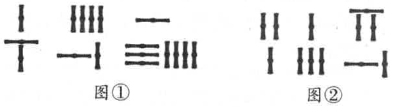
\includegraphics[width=0.6\linewidth]{pic/20200531005.png}\\
\begin{solution}
    \(\begin{cases} 2x+y=7\\ x+3y=11\end{cases}; x=2,y=3\)
\end{solution}
\item 亚洲文明对话大会召开期间,大批的大学生志愿者参与服务工作.某大学计划组织本校全体志愿者统一乘车去会场,若单独调配36座新能源客车若干辆,则有2人没有座位;若只调配22座新能源客车,则用车数量将增加4辆,并空出2个座位.\\
    (1)计划调配36座新能源客车多少辆?该大学共有多少名志愿者?\\
    (2) 若同时调配36座和22座两种车型,既保证每人 有座,又保证每车不空座,则两种车型各需多少辆?
\begin{solution}
        (1)设\(n\)辆36座车,则\(36n+2=22(n+4)-2 \Rightarrow n=6\),\(\therefore \)36座6辆,共有218名志愿者.\\
        (2)设36座m辆,22座n辆,得:\(\begin{cases} 36m+22n=218\\ 18m+11n=109\end{cases}\)
\end{solution}

\item 已知一个锐角的余角是这个锐角的补角的\(\frac{1}{4}\).求这个锐角的度数.
\begin{solution}
        解:设这个锐角的度数为x.
        由题意得\(90-x=\frac{1}{4}(180-x)\)解得\(x=60\).
        答:所求锐角为\(60 ^\circ\) .
\end{solution}
\item 一个两位数,个位上的数是十位上的数的2倍, 个位与十位上的数的和比这个两位数少36,求这个两位数.
\begin{solution}
        解:设十位上的数字为\(x\),则个位上的数字为\(2x\),这个两位数为\(10x+2x\),根据题意得\(x+2x+36=10x + 2x\),得\(x=4\).\\
        个位上的数为\(2x=8\).所以\((10x + 2x)=48\).
\end{solution}
\item  A,B两地相距120 km,甲骑车每小时走15 km,乙骑车每小时比甲慢3 km\\
    (1)甲、 乙从A地同向而行,试问:\\
 \ding{172}若甲、乙同时出发,问5 h后,甲、乙相距多少km?\\
 \ding{173}若乙先走3 h,问甲多少小时后追上乙?\\
 \ding{174} 乙先出发2 h,若甲要在84 km处追上乙,问甲每小时比原来要多走多少km?\\
(2)甲、乙相向而行, 试问:\\
 \ding{172} 甲、乙何时相遇,这时距A多少km?\\
 \ding{173}若甲、乙骑一个来回,第二次何时相遇,这时距A多少km?\\
 \ding{174} 甲、乙第一次相距30 km和第二次相距30 km所用的时间分别为多少小时?\\
\begin{solution}
     解: (1)甲、 乙同向而行.\\
     \ding{172}设甲、乙相距\(x\)(km).\\
         \(x=75 - 60, x=15.\)\\
         \ding{173} 设\(x\)小时后甲追上乙.有:\(15x一(36+12x)=0 , x=12\).\\
     当\(x=12h,S_\text{甲} =12X15=180 km\),与题意不符(因为A,B相距120 km),即甲不可能追上乙.故本题无解.\\
     \ding{174} 设甲每小时比乙多走\(x km\),而乙走\(84 km\)要\(7h\),就是说乙先走\(2h\)后, 甲走\(5h\)追上乙.\\
     所以\(5x=24,x=4.8\),又因为甲原来每\(h\)比乙快3 km,所以甲要在84 km处追上乙, 需每\(h\)比原来快\(1.8 km\).\\
     (2)甲、 乙相向而行.\\
     设\(t\)小时后甲、乙相遇.得 \(15t+12t=120 \Rightarrow t=\frac{40}{9}\),所以\(s_\text{甲} =66\frac{2}{3}\).\\
     \ding{173}甲、 乙1 h共走27 km,第二次相遇时所走路程是360 km,故共走\(\frac{360}{27}=\frac{40}{3}\)h\\
     \(S_\text{甲}=200, S_\text{甲}'=240-200=40\)\\
     答:\(\frac{40}{3}\)h后, 甲、 乙第二次相遇, 此时距离A地40 km\\
     \ding{174} 甲、 乙1 h共走27km,走90 km需\(\frac{10}{3}\)小时,即相距30 km时为出发后\(\frac{10}{3}\)h.第二次相距30km时甲、乙已走了150 km.需用\(\frac{150}{27}=\frac{50}{9}\)h
\end{solution}
\item  一台机器的检修工程, 甲组单独做需要8 h完成, 乙组单独做需6 h完成, 现由甲、 乙的组合做2 h后.再由乙单独做完,共需几h才能完成这台机器的检修工作?
\begin{solution}
        设完成机器的检修工作共需x小时, 得\((\frac{1}{8}+\frac{1}{6}\times 2+\frac{x-2}{6}=1 \Rightarrow x=\frac{9}{2}\)
\end{solution}
\item 八一商场某种上衣因换季准备打折出隽, 若按原价七五折出售将赔25元,而按原价的九折出售将赚20元, 试问这种上衣的原价是多少?
\begin{solution}
        解:设这种上衣的原价是x元.根据题意得 \(0.75x + 25=0.9x-20 \Rightarrow x=300\)
\end{solution}
\item 浓度为18\%的盐水一桶.加入50 kg水后, 浓度变为15\%.求原有盐水多少千克?
\begin{solution}
        解:设原有盐水\(x\)kg,列方程为\(\frac{15}{100}(x+50)=\frac{18}{100}x \Rightarrow x=250\)
\end{solution}
\item 已知关于x的方程\(\frac{x+a}{x-2}=-1\)的根大于0,求\(a\)的取值范围.
\begin{solution}
        方程\(\frac{x+a}{x-2}=-1\)可化为\(x+a=2-x\),即\(x=\frac{2-a}{2}\)\\
        因为方程的根大于0,所以\(\frac{2-a}{2}>0 \Rightarrow a<2\)\\
        又\(x-2 \ne 0 \Rightarrow \frac{2-a}{2}\ne 2 \Rightarrow a\ne -2\)\\
        所以a的取值范围:\(a<2\)且\(a \ne -2\).
\end{solution}
\item 一年期定期储蓄年利率为2.25\%,所得利息要交纳20\%的利息税, 已知某储户将一笔钱以一年期定期储蓄, 到期纳税后得利息450元, 问该储户存入多少本金?
\begin{solution}
        设该储户存入\(x\)元钱, 得\(2.2\%(l-20\%)x=450\),解得\(r=25 000\).
\end{solution}
\item 当\(m\)取何值时, 方程\(3x-mx+l= 2x + 9\)的解为2.
\begin{solution}
        解:把 x=2 代入 \(3x-mx+l=2x + 9\),得 \(6-2m+l≡4 + 9\).  移项, 得\(-2m=4+9-7 \Rightarrow m=-3\),
\end{solution}
\item 解关于\(y\)的方程,\((k^2+2k+3)y=3(y+2)+k\)
\begin{solution}
        \((k^2+2k+3)y=3(y+2)+k\)整理, 得\((k^2+2k)y=2+k \Rightarrow k(k+2)y=2+k\)\\
        当\(k=-2\)时, 方程有无数多个解, 当\(k \ne -2\)时,得\(ky=1\).
        所以当\(k\ne -2\)且\(k \ne 0\)时, 方程的解为\(y=\frac{1}{k}\),当\(k=0\)时,原方程无解.
\end{solution}
\item 巳知方程\(2|x|-k= kx-3\)无负数解, 那么\(k\)的取值范围是什么?
\begin{solution}
        若有负数解,方程化为\(-2x-k=kx-3 \Rightarrow x=\frac{k-3}{-2-k}<0 \Rightarrow k>3\text{或}k<-2\)
        所以\(-2\le k\le 3\)时方程无负数解.
\end{solution}
\item 若\(a>0,b<0\),则方程\(|x-a| + |x-b| =a-b\)的解集是什么?
\begin{solution}
        当\(x\ge a\)时, 原方程化为\(x-a+x-b=a-b \Rightarrow x=a\)\\
        当\(b<x<a\)时, 原方程化为\(a-x+x-b=a=a-b \Rightarrow 0=0\),所以满足\(b<x<a\)任何有理敷都为方程的解,\\
        当\(x\le b\)时, 原方程化为\(x-a+b-x=a-b \Rightarrow x=b\),\\
        综上所述,解集是\(b\le x\le a\).
\end{solution}
\item 巳知方程\(|x|=ax+1\)有一个负根而没有正根,那么\(a\)的取值范围是什么?
\begin{solution}
        因为方程有一个负根而没有正根, 所以\(x<0\)\\\\
        所以\(|x|=ax+1\)去绝对值后,化为\(-x=ax+1 \Rightarrow (-1-a)x=1\)\\
        当\(-1-a=0\)时, 方程无解,\\
        当 \(-1-a\ne 0\)时,\(x=\frac{1}{-1-a}\)
        由条件\(x=\frac{1}{-1-a}\),所以\(a>-1\)
\end{solution}
\end{liti}

\section{中考真题}%

\subsection{类型:解一次方程组(10年2考,均为方程组的解法)}%
\begin{zhenti}[resume]
\item  (2011江西12题3分)方程组\(\begin{cases} 2x+y=5\\ x-y=7\end{cases}\)的解是\tkt{\(\begin{cases} x=4\\ y=-3\end{cases}\)}
\item  (2016江西13(1)题3分)解方程组:\(\begin{cases} x-y=2\\ x-y=y+1\end{cases}\)
\begin{solution}
        \(x=3,y=1\)
\end{solution}
\end{zhenti}

\subsection{一次方程(组)的实际应用(10年9考)}%
\subsubsection{购买分配类问题(10年5考)}%

\begin{zhenti}[resume]
\item  (2010江西13题3分)某班有40名同学去看演出,购买甲、乙两种票共用去370元,其中甲种票每张10元,乙种票每张8元.设购买了甲种票\(x\)张,乙种票\(y\)张,由此可列出方程组: \tkt{\(\begin{cases} x+y=40\\ 10x+8y=370\end{cases}\)}  .
\item  (2013江西9题3分)某单位组织34人分别到井冈山和瑞金进行革命传统教育,到井冈山的人数是到瑞金的人数的2倍多1人,求到两地的人数各是多少?设到井冈山的人数为\(x\)人,到瑞金的人数为\(y\)人,请列出满足题意的方程组\tkt{\(\begin{cases} x+y=34\\ x=2y+1\end{cases}\)}  .
\item  (2018江西9题3分)中国的《九章算术》是世界现代数学的两大源泉之一,其中有一问题:``今有牛五、羊二,直金十两 . 牛二、羊五,直金八两 . 问牛羊各直金几何?''译文:今有牛5头,羊2头,共值金10两;牛2头,羊5头,共值金8两.问牛、羊每头各值金多少?设牛、羊每头各值金\(x\)两、\(y\)两,依题意,可列出方程组为 \tkt{\(\begin{cases} 5x+2y=10\\ 2x+2y=8\end{cases}\)}.
\item (2014江西16题6分)小锦和小丽购买了价格分别相同的中性笔和笔芯.小锦买了\( 20\)支笔和\(2\)盒笔芯,用了\( 56\)元;小丽买了\( 2\)支笔和\(3\)盒笔芯,仅用了\( 28\)元,求每支中性笔和每盒笔芯的价格.
\begin{solution}
    设中性笔和笔芯的价格分别为\(x,y\)元.\\
    \(\begin{cases} 20x+2y=56\\ 2x+3y=28\end{cases}\Rightarrow \begin{cases} x=2\\ y=8\\  \end{cases}\)\\
\end{solution}
\item  (2010江西21题8分)剃须刀由刀片和刀架组成.某时期,甲、乙两厂家分别生产老式剃须刀(刀片不可更换)和新式剃须刀(刀片可更换) \cdot 有关销售策略与售价等信息如下表所示:
\begin{table}[H]
  \centering
    \begin{tabular}{|c|c|c|c|}
    \hline
    \multirow{2}[4]{*}{} & \multirow{2}[4]{*}{老式剃须刀} & \multicolumn{2}{c|}{新式剃须刀} \bigstrut\\
\cline{3-4}          &       & 刀架    & 刀片 \bigstrut\\
    \hline
    售价    & 2.5(元/把) & 1(元/把) & 0.55(元/片) \bigstrut\\
    \hline
    成本    & 2(元/把) & 5(元/把) & 0.05(元/片) \bigstrut\\
    \hline
    \end{tabular}%
\end{table}%
某段时间内,甲厂家销售了8400把剃须刀,乙厂家销售的刀片数量是刀架数量的50倍,乙厂家获得的利润是甲厂家的两倍,问这段时间内乙厂家销售了多少把刀架?多少片刀片?
\begin{solution}
    设刀架\(x\)片, \(-4x + 0.5\times 50x = 2\times 0.5\times 8400\),得到:刀架400,刀片20000
\end{solution}
\item 《九章算术》是中国传统数学最重要的著作之一,书中记载:``今有人共买鸡,人出九,盈十一;人出六,不足十六,问人数几何? ''意思是:``有若干人共同出钱买鸡,如果每人出九钱,那么多出了十一钱;如果每人出六钱,那么少了十六钱.问:共有几个人?''设共有\(x\)个人共同出钱买鸡,根据题意,可列一元一次方程为 \tkt{ \(9x-11=6x+16\)}  .
\item  (2019娄底)某商场用14500元购进甲、乙两种矿泉水共500箱,矿泉水的成本价与销售价如下表所示
\begin{table}[H]
  \centering
    \begin{tabular}{|c|c|c|}
    \hline
    类别    & 成本价(元/箱) & 销售价(元/箱) \bigstrut\\
    \hline
    甲     & 25    & 35 \bigstrut\\
    \hline
    乙     & 35    & 48 \bigstrut\\
    \hline
    \end{tabular}%
\end{table}%
求:(1)购进甲、乙两种矿泉水各多少箱?\\
(2)该商场售完这500箱矿泉水,可获利多少元?\\
\begin{solution}
\(\begin{cases} x+y=500\\ 25x+35y=14500 \end{cases}\),得到:(1)甲300,乙200; (2)获利5600
\end{solution}
\end{zhenti}

\subsubsection{实物模型问题}%
\begin{zhenti}[resume]
\item  (2012江西20题8分)小华写信给老家的爷爷,问候``八一''建军节.折叠长方形信纸,装入标准信封时发现:若将信纸如图 \ding{172}连续两次对折后,沿着信封口边线装入时,宽绰有3. 8 cm;若将信纸如图 \ding{173}三等分折叠后,同样方法装入时,宽绰1.4 cm.试求信纸的纸长与信封的口宽.
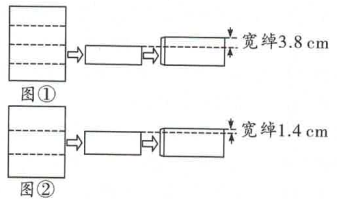
\includegraphics[width=0.5\linewidth]{pic/20200531002.png}
\begin{solution}
        长\(x\), 宽\(y:\) \(\begin{cases} \frac{y-x}{4}=3.8\\ \frac{y-x}{3}=1.4 \end{cases}\);长28.8,宽11
\end{solution}
\item  (2011江西20题8分)有一种用来画圆的工具板(如图所示),工具板长21 cm,上面依次排列着大小不等的五个圆(孔),其中最大圆的直径为3 cm,其余圆的直径从左到右依次递减0.2 cm.最大圆的左侧距工具板左侧边缘1.5 cm,最小圆的右侧距工具板右侧边缘1.5 cm,相邻两圆的间距\(d\)均相等.\\
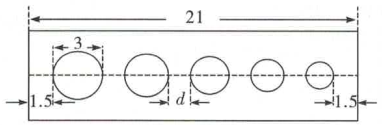
\includegraphics[width=0.5\linewidth]{pic/20200531003.png}\\
(1)直接写出其余四个圆的直径;\\
(2)求相邻两圆的间距.
\begin{solution}
    (1) 2.8, 2.6, 2.4, 2.2\\
    (2) \(d=\frac{5}{4}\)
\end{solution}
\item  (2016江西19题8分)如图是一根可伸缩的鱼竿,鱼竿是用10节大小不同的空心套管连接而成.闲置时鱼竿可收缩,完全收缩后,鱼竿长度即为第1节套管的长度(如图 \ding{172}所示);使用时,可将鱼竿的每一节套管都完全拉伸(如图 \ding{173}所示).图 \ding{174}是这根鱼竿所有套管都处于完全拉伸状态下的平面示意图.已知第】节套管长50 cm,第2节套管长46 cm,依此类推,每一节套管均比前一节套管少4 cm.完全拉伸时,为了使相邻两节套管连接并固定,每相邻两节套管间均有相同长度的重叠,设其长为\(x\) cm.\\
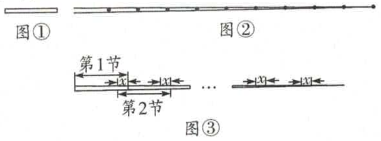
\includegraphics[width=0.7\linewidth]{pic/20200531004.png}\\
(1) 请直接写出第5节套管的长度;\\
(2) 当这根鱼竿完全拉伸时,其长度为311 cm,求\(x\)的值.
\begin{solution}
    (1)第5节套管 34cm;\\
    (2)\(x=1\)
\end{solution}
\end{zhenti}


\subsubsection{核心素养}%
\begin{zhenti}[resume]
\item 一道习题:“从甲地到乙地有一段上坡与一段平路,如果保持上坡每小时走3 km,平路每小时走4 km,下坡每小时走5 km,那么从甲地到乙地需 54 min,从乙地到甲地需42 min.甲地到乙地全程是多少?”小红将这个实际问题转化为二元一次方程组问题.设未知数\(x,y\),已经列出一个方程\(\frac{x}{3}+\frac{y}{4}=\frac{54}{60}\),则另一个方程正确的是(\qquad)\\
\begin{tasks}(4)
\task \(\frac{x}{4}+\frac{y}{3}=\frac{42}{60}\)
\task \(\frac{x}{5}+\frac{y}{4}=\frac{42}{60}\)
\task \(\frac{x}{4}+\frac{y}{5}=\frac{42}{60}\)
\task \(\frac{x}{3}+\frac{y}{4}=\frac{42}{60}\)
\end{tasks}
\begin{solution}
    B
\end{solution}
\item 如图,约定:上方相邻两数之和等于这两数下方箭头共同指向的数.\\
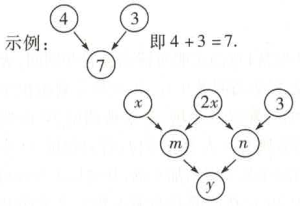
\includegraphics[width=0.5\linewidth]{pic/20200531006.png}\\
则(1)用含\(x\)的式子表示\(m=\)\tkt{\(3x\)};\\
(2)当\(y=-2\)时,\(n\)的值为\tkt{\(1\)}.
\item 用消元法解方程组\(\begin{cases} x-3y=5, & \text{\ding{172}}\\ 4x-3y=2 \text{\ding{173}}\end{cases}\)时,两位同学的解法如下:\\
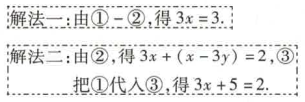
\includegraphics[width=0.4\linewidth]{pic/20200531007.png}\\
(1)反思:上述两个解题过程中有无计算错误?并说明原因;\\
(2)请选择一种你喜欢的方法,完成解答.
\begin{solution}
    (1)解法一有误,\ding{172}-\ding{173}得: \(-3x=3\)\\
    (2)\(x=-1, y=-2\)
\end{solution}
\end{zhenti}

\subsubsection{数学文化专练}%
\begin{enumerate}
    \item 《九章算术》:方程术\\
《九章算术》是中国传统数学最重要的著作,奠定了中国传统数学的基本框架,它的代数成就主要包括开方术、正负术和方程术,其中,方程术是《九章算术》最高的数学成就,书中收集了246个与生产、生活实践有联系的应用问题.

\item 《孙子算经》:方程\\
《孙子算经》是中国古代重要的数学著作,成书大约在四、五世纪,也就是大约一千五百年前,传本的《孙子算经》共三卷,上卷叙述算筹记数的纵横相间制度和筹算乘除法,中卷举例说明等筹算分数算法和筹算开平方法.下卷第31题,可谓是后世``鸡兔同笼''题的始祖,后来传到日本,变成``鹤龟算''.
\end{enumerate}
\begin{zhenti}[resume]
\item 《九章算术》是我国古代数学名著,卷七``盈不足''中有题译文如下:今有人合伙买羊,每人出5钱,会差45钱;每人出7钱.会差3钱.问合伙人数、 羊价各是多少?设合伙人数为\(x\)人,所列方程正确的是(\qquad)\\
\begin{tasks}(2)
\task \(5x-45=7x-3\)
\task \(5x+45=7x+3\)
\task \(\frac{x+45}{5}=\frac{x+3}{7}\)
\task \(\frac{x-45}{5}=\frac{x-3}{7}\)
\end{tasks}
\begin{solution}
    B
\end{solution}
\item 《孙子算经》是中国传统数学的重要著作.其中有一道题,原文是:``今有木,不知长短,引绳度之,余绳四尺五寸;屈绳量之,不足一尺,木长几何? ''意思是:用一根绳子去量一根木头的长,绳子还剩余4.5尺;将绳子对折再量木头,则木头还剩余1尺,问木头长多少尺?可设木头长为x尺,绳子长为y尺,则所列方程组正确的是(\qquad)\\
\begin{tasks}(4)
\task \(\begin{cases} y=x+4.5\\ 0.5y=x-1\end{cases}\)
\task \(\begin{cases} y=x+4.5\\ y=2x-1\end{cases}\)
\task \(\begin{cases} y=x-4.5\\ 0.5y=x+1\end{cases}\)
\task \(\begin{cases} y=x-4.5\\ y=2x+1\end{cases}\)
\end{tasks}
\begin{solution}
    A
\end{solution}
\end{zhenti}

\section{强化训练}%

\subsection{综合题组1}%
(30分钟)
\begin{shiti}
\item 基础过关
    \begin{shiti}[resume]
    \item 一元一次方程\(x-2=0\)的解是(\tkt{A})\\
    \begin{tasks}(4)
    \task \(x-2\)
    \task \(x=-2\)
    \task \(x=0\)
    \task \(x=1\)
    \end{tasks}
\item 方程组\(\begin{cases} 3x+2y=7\\ 6x-2y=11\end{cases}\)(\tkt{D})\\
\begin{tasks}(2)
\task \(\begin{cases} x=-1\\ y=5\end{cases}\)
\task \(\begin{cases} x=1\\ y=2\end{cases}\)
\task \(\begin{cases} x=3 \\ y=-1\end{cases}\)
\task \(\begin{cases} x=2\\ y=\frac{1}{2}\end{cases}\)
\end{tasks}
\item 已知九年级某班30位同学种树72棵,男生每人种3棵树,女生每人种2棵树,设男生有\(x\)人,则 (\tkt{D})\\
    \begin{tasks}(2)
 \task  \(2x+3(72-x) =30\)
 \task  \(3x+2(72 -x) =30\)
 \task  \(2x+3(3O-x) =72\)
 \task  \(3x +2(30-x) =72\)
 \end{tasks}
\item 某活动小组购买了 4个篮球和5 个足球,一共花费了 466元,其中篮球的单价比足球的单价多4元,求篮球的单价和足球的单价.设篮球的单价为\(x\)元.足球的单价为\(y\)元,那么根据题意,下列方程组中,正确的是 (\tkt{B})\\
    \begin{tasks}(4)
        \task \(\begin{cases} 4x+5y=466\\ x+4=y\end{cases}\)
        \task \(\begin{cases} 4x+5y=466\\ x-4=y\end{cases}\)
        \task \(\begin{cases} 5x+4y=466\\ x-4=y\end{cases}\)
        \task \(\begin{cases} 5x+4y=466\\ x+4=y\end{cases}\)
    \end{tasks}
\item 学校计划购买A和B两种品牌的足球,已知一个A品牌足球60元.一个B品牌足球75元.学校准备将1500元钱全部用于购买这两种足球(两种足球都买),该学校的购买方案共有 (\tkt{B})\\
    \begin{tasks}(4)
 \task  3种  \task  4种  \task  5种  \task  6种
 \end{tasks}
\item 已知关于\(x,y\)的方程组\(\begin{cases} x+2y=k-1\\ 2x+y=5k+4\end{cases}\)的解满足\(x+y=5\),则k的值为\tkt{\(2\)}
\item  某校八年级共有160名学生,在一次模拟考试中.他们的成绩优秀率(成绩在90分以上)为28\%.如果女生的成绩优秀率为4\%,男生的成绩优秀率为36\%,求八年级男生、女生各有多少名学生?设男生为\(x\)名.女生为\(y\)名,根据题意列关于\(x,y\)的方程组为 \tkt{\(\begin{cases} x+y=160\\ 4\%\cdot y+36\%\cdot x=28\%\times 160 \end{cases}\)}.
\item 用1块A型钢板可制成4件甲种产品和1件乙种产品;用1块B型钢板可制成3件甲种产品和2件乙种产品.要生产甲种产品37件,乙种产品18件,则恰好需用A,B两种型号的钢板共\tkt{\(11\)}块.
\item 数学文化:我国古代的数学名著《九章算术》中有下列问题:``今有女子善织,日自倍,五日织五尺.问日织几何?''其意思为:今有一女子很会织布,每日加倍增长,5日共织布5尺.问每日各织多少布?根据此问题中的已知条件,可求得该女子第一天织布 \tkt{\(\frac{5}{31}\)}  尺.
\item 某品牌旗舰店平日将某商品按进价提高4\%后标价,在某次电商购物节中,为促销该商品,按标价8折销售,售价为2240元,则这种商品的进价是 \tkt{2000}元.
\item 解方程:\(\frac{x-3}{2}-\frac{2x+1}{3}=1\)
\begin{solution}
        \(x=-17\)
\end{solution}
\item 解方程组:\(\begin{cases} x+3y=6\\ 2x+y=7\end{cases}\)
\begin{solution}
        \(x=3,y=1\)
\end{solution}
\item 小甘到文具超市去买文具,请你根据下图中的对话信息,求中性笔和笔记本的单价分别是多少元?\\
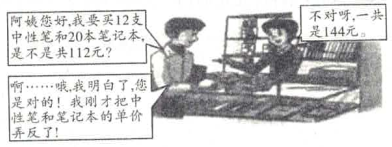
\includegraphics[width=0.7\linewidth]{pic/20200531008.png}
\begin{solution}
    中性笔2元,笔记本6元.
\end{solution}
\item 为实施乡村振兴战略,解决某山区老百姓出行难问题,当地政府决定修建一条高速公路,其中一段长为146米的隧道贯穿工程由甲乙两个工程队负责施工,甲工程队独立工作2天后,乙工程队加入,两工程队又联合工作了 1天,这3天共掘进26米.已知甲工程队每天比乙工程队多掘进2米,按此速度完成这项隧道贯穿工程,甲乙两个工程队还需联合工作多少天?
\begin{solution}
        10 天
\end{solution}
\item  某公司用火车和汽车运输两批物资.第一批次用2节火车车皮和5辆汽车运送物资130吨;第二批次用4节火车车皮和3辆汽车运送物资218吨,试问每节火车车皮和每辆汽车平均各装物资多少吨?
\begin{solution}
        火车50, 汽车6
\end{solution}
\item 如图 \ding{172},是某单位的透空护栏,图 \ding{173}是它的示意图,它是用外径为3 cm的圆钢管与外圆直径为15 cm的圆圈焊接而成的(圆圈由扁直钢筋做成,厚度忽略不计.两圆钢管之间夹一个圆圈),若要做高度统一为2 m.K为7.4∣ m的护栏.试问:需要展直扁钢筋和圆钢管的总长度各是多少米?\\
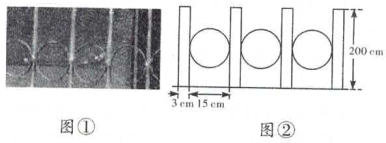
\includegraphics[width=0.6\linewidth]{pic/20200531009.png}
\begin{solution}
    直钢筋\(6.15\pi \)m, 圆钢管\(84\)m
\end{solution}
\end{shiti}
\item 满分冲关
    \begin{shiti}[resume]
    \item 如图是一个最简单的二阶幻圆的模型,要求: \ding{172}内、外两个圆周上的四个数字之和相等; \ding{173}外圆两直径上的四个数字之和相等,则图中两空白圆圈内应填写的数字从左到右依次为 \tkt{2}和\tkt{9}.\\
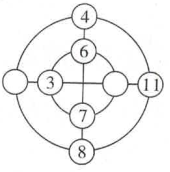
\includegraphics[width=0.2\linewidth]{pic/20200531010.png}
    \item 数学文化:``今有善行者行一百步,不善行者行六十步''(出自《九章算术》)意思是:同样时间段内,走路快的人能走100步,走路慢的人只能走60步,假定两者步长相等,据此回答以下问题:\\
(1) 今不善行者先行一百步,善行者追之,不善行者再行六百步,问孰至于前,两者几何步隔之?即:走路慢的人先走100步,走路快的人开始追赶,当走路慢的人再走600步时,请问谁在前面,两人相隔多少步?\\
(2) 今不善行者先行两百步,善行者追之,问几何步及之?即:走路慢的人先走200步,请问走路快的人走多少步才能追上走路慢的人?
\begin{solution}
    (1)走路快的在前,相隔300步; (2)走路快的要走500步才能追上.
\end{solution}
\end{shiti}
\end{shiti}
\end{document}
